% This is the aspauthor.tex LaTeX file
% Copyright 2010, Astronomical Society of the Pacific Conference Series

\documentclass[11pt,twoside]{article}

\usepackage{asp2010}

%\setlength{\textfloatsep}{2pt}
%\setlength{\floatsep}{8pt}
\resetcounters

%\bibliographystyle{asp2010}

\markboth{Yihan Song, Ali Luo, and Yongheng Zhao}{A New Python Library --- PydasLib}

\begin{document}

\title{A New Python Library for Spectroscopic Analysis with MIDAS Style}
\author{Yihan Song$^{1,2}$, Ali Luo$^{1,2}$, and Yongheng Zhao$^{1,2}$
\affil{$^1$Key Laboratory of Optical Astronomy, Nationsal Astronomical obervatories, Chinese Academy of Sciences, 20A Datun Road, Chaoyang District, Beijing, 100012, China}
\affil{$^2$National Astronomical Observatories, Chinese Academy of Sciences,20A Datun Road, Chaoyang District, Beijing, 100012, China}
}

\begin{abstract}
The ESO MIDAS is a system for astronomiers to analyze data and many 
astronomiers are using that. Python is a high level script language and 
there are many applications in astronomyical data process. 
We release a new python library which realize some MIDAS commands in python.
People can use it to write a MIDAS style python code. We call it PydasLib.
It is a python library based on ESO MIDAS functions, which is 
easily used by astronomiers who is familiar with the useage of MIDAS.
\end{abstract}

	  \section{Introduction}
As a popular language, Python is wildly used in astronomical programming now. 
More and more researchers use python to realize their algorithm and ideas for 
astronomical data processing. 

MIDAS is an outstanding programming language in astronomy. It is created and 
maintained by by European Organisation for Astronomical Research in the 
Southern Hemisphere (ESO). 
There are a lot of good codes written in MIDAS and there are a lot of people 
use it for years.

We release a new python library which realize some MIDAS commands in python.
People can use it to write a MIDAS style python code. We call it PydasLib.
Our work here can help two kinds of people:
\begin{itemize}
   \item Python users who want to migrate some MIDAS codes to python. 
   \item MIDAS users who want to use python to realize their idea using commands which 
they are familiar with.
\end{itemize}

%            \vfill
%           \begin{block}{Abstract}
%The ESO MIDAS is a system for astronomiers to analyze data and many 
%astronomiers are used to that. Python is a high level script language and 
%there are many applications in astronomyical data process. 
%A new Python library is built based on ESO MIDAS functions, which is 
%easily used by astronomiers who is familiar with the useage of MIDAS. This 
%library helps people to migrate there favorate MIDAS code to python code.
% 
%           \end{block}

          \section{MIDAS and Python}
\subsection{ESO MIDAS}

ESO MIDAS is a system which provides general tools for image processing 
and data reduction with emphasis on astronomical applications including 
imaging and special reduction packages. Many astronomy researchers use 
this system to achieve their thought and algorithms on data analysis. 
The MIDAS supports many basic data types and functions such as fitting, 
statistics on tables and images etc. It can also display images 
and output the results to a file or on a screen. \\

There are four shortness of the MIDAS:
\begin{itemize}
  \item  Data structure 
in MIDAS is not very flexible. The basic type of variable in MIDAS can be 
integer, float or string. There are no list or dictionary in it. 
   \item  
MIDAS is a self-sealing system. The code can be run very well under 
its environment but it is not able to be called by other programs. It 
is hard to write a function in MIDAS which serves the whole software 
pipeline. 
   \item  It is not convenient to run the MIDAS code
 in parallel.    You need to select parallel mode in the system to run 
another MIDAS program at the same time. Nowadays, with a great deal of data
 springing up, how long will a program take will be considered.  
    \item MIDAS can not be installed in Windows which limits its
applications. 
\end{itemize}

          \subsection{Python}
Python is an interpreted, general-purpose high-level programming language 
whose design philosophy emphasizes code readability. It supports multiple 
programming paradigms, primarily but not limited to object oriented, 
imperative and, to a lesser extent, functional programming styles. It 
features a fully dynamic type system and automatic memory management. 

          \subsection{PyMidas}
PyMidas is a a product of ESO project named Sampo since 2005. It is 
an interface for python call MIDAS programs. Because the precondition of 
using PyMidas is that MIDAS should be installed, it is hard to use under
different operation system.
%Because of python's advantage, ESO has started a project named Sampo since 2005. 
%The first sub-project of Sampo is PyMidas. It provides an interface from 
%Python scripting language to the ESO-MIDAS astronomical data processing 
%system. It allows a user to exploit both the rich legacy of MIDAS software 
%and the power of Python scripting in a unified interactive environment. When 
%you run a PyMidas program including some MIDAS commands, the PyMidas will 
%call MIDAS which runs in the background. That means you can not execute a 
%PyMidas code without MIDAS system, and some limits of MIDAS will be introduced 
%to PyMidas.

          \section{PydasLib --- Our work}
In PydasLib, we fulfill dozens of MIDAS commands in python. 
The goal of our work is to make a library of python which 
can achieve the function of some MIDAS commands. Using this library, people 
can write their algorithms in python without MIDAS or migrate best MIDAS
codes to python. The code can be easily 
called by other programs under different operation system. 

	  \subsection{PydasLib Commands and Corresponding MIDAS Commands}
Table \ref{commands} shows PydasLib commands and the corresponding MIDAS commands.
The function of PydasLib commands are almost as same as the corresponding MIDAS ones.
Table \ref{new-commands} shows commands which are not included in MIDAS. 

\begin{table}[!hb]
\begin{center}
\caption{Commands list}
\label{commands}
\begin{tabular}{cc||cc}
\hline
 PydasLib & MIDAS &PydasLib & MIDAS\\
\hline
\hline
 centerGauss & center/gauss &
computeFit & compute/fit \\
computeImage & compute/fit &
computeTable & compute/table\\
convertTable & convert/table  &
convolveImage & convolve/image\\
copyDD & copy/dd &
copyDK & copy/dk\\
copyIT & copy/it &
copyTable & copy/table\\
cp & cp &
createColumn & create/column\\
createImage & create/image &
createTable & create/table\\
deleteColumn & delete/column &
deleteDescriptor & delete/descriptor\\
deleteTable & delete/table &
exists & exists \\
extractImage & extract/image &
fitImage & fit/image\\
fitTable & fit/table &
insertImage & insert/image\\
intapeFits & intape/fits &
interpolateTI & interpolate/ti\\
mergeTable & merge/table &
nameColumn & name/column\\
outputi & outputi &
outputr & outputr\\
overplot & overplot &
plot & plot\\
readImage & read/image &
renameTable & rename/table\\
selectFunction & select/function &
selectTable & select/table\\
sortTable & sort/table &
statisticsImage & statistics/image\\
statisticsTable & statistics/table &
value &value \\
writeDescriptor & write/descriptor\\
\hline 
\hline
\end{tabular}
%% Any table notes must follow the \end{tabular} command.
%\tablenotetext{a}{Sample footnote for table~\ref{tbl-2} that was
%generated with the \LaTeX\ table environment}
%\tablenotetext{b}{Yet another sample footnote for table~\ref{tbl-2}}
%\tablenotetext{c}{Another sample footnote for table~\ref{tbl-2}}
%\tablecomments{We can also attach a long-ish paragraph of explanatory
%material to a table.}
\end{center}
\end{table}

\begin{table}[!hb]
\begin{center}
\caption{New Commands list}
\label{new-commands}
\begin{tabular}{c|c}
\hline
 PydasLib & Comments\\
\hline 
\hline
 add\_fit  & add a fitting function to the fitting file\\
del\_fit & remove a fitting function from the fitting file \\
get\_global\_key & get a handle of a image, table or fitting file\\
savefig &  save the figure as a file\\
valid\_row & return a list of valid rows of the table\\
\hline
\hline
\end{tabular}
%% Any table notes must follow the \end{tabular} command.
%\tablenotetext{a}{Sample footnote for table~\ref{tbl-2} that was
%generated with the \LaTeX\ table environment}
%\tablenotetext{b}{Yet another sample footnote for table~\ref{tbl-2}}
%\tablenotetext{c}{Another sample footnote for table~\ref{tbl-2}}
%\tablecomments{We can also attach a long-ish paragraph of explanatory
%material to a table.}
\end{center}
\end{table}
          \section{Example }%--- A part of a simple code using PydasLib}
Table \ref{code} shows a short example. The example uses PydasLib to read a Sloan fits file, to make a convolution with gaussion profile and to extract H$\alpha$ emission line. Finally, the example save the plotted figures(Figure:\ref{fig}) into files.

\begin{table}[!hb]
\begin{center}
\caption{Example Code}
\label{code}
\begin{tabular}{cl}
lineno & code\\
\hline
8 & intapeFits(1, "Sloa", "data.fit")  \\
14 & spsl0001 = extractImage (Sloa0001, [1, npixsloan, 1], type='pixel', \\
  & name="spsl0001")\\
29 & redshift = copyDK('Sloa0001', 'Z')  \\
45 & name\_zzero = convertTable ('name\_zzero', [spsl\_tab,'lambda\_zero',\\
   & 'fluxdens'], refmidsloan, 'spline')\\
48 & plot(name\_zzero)\\
56 & conv = convolveImage(img1, psf, 'conv') \\
57 & plot(conv)\\
61 & halpha = extractImage (name\_zzero, [6500,6630],name="halpha") \\
62 & plot(halpha)\\
\end{tabular}
\end{center}
\end{table}
	 
\begin{figure}[!hb]
\begin{center}
\caption{Figures of the example}
\label{fig}
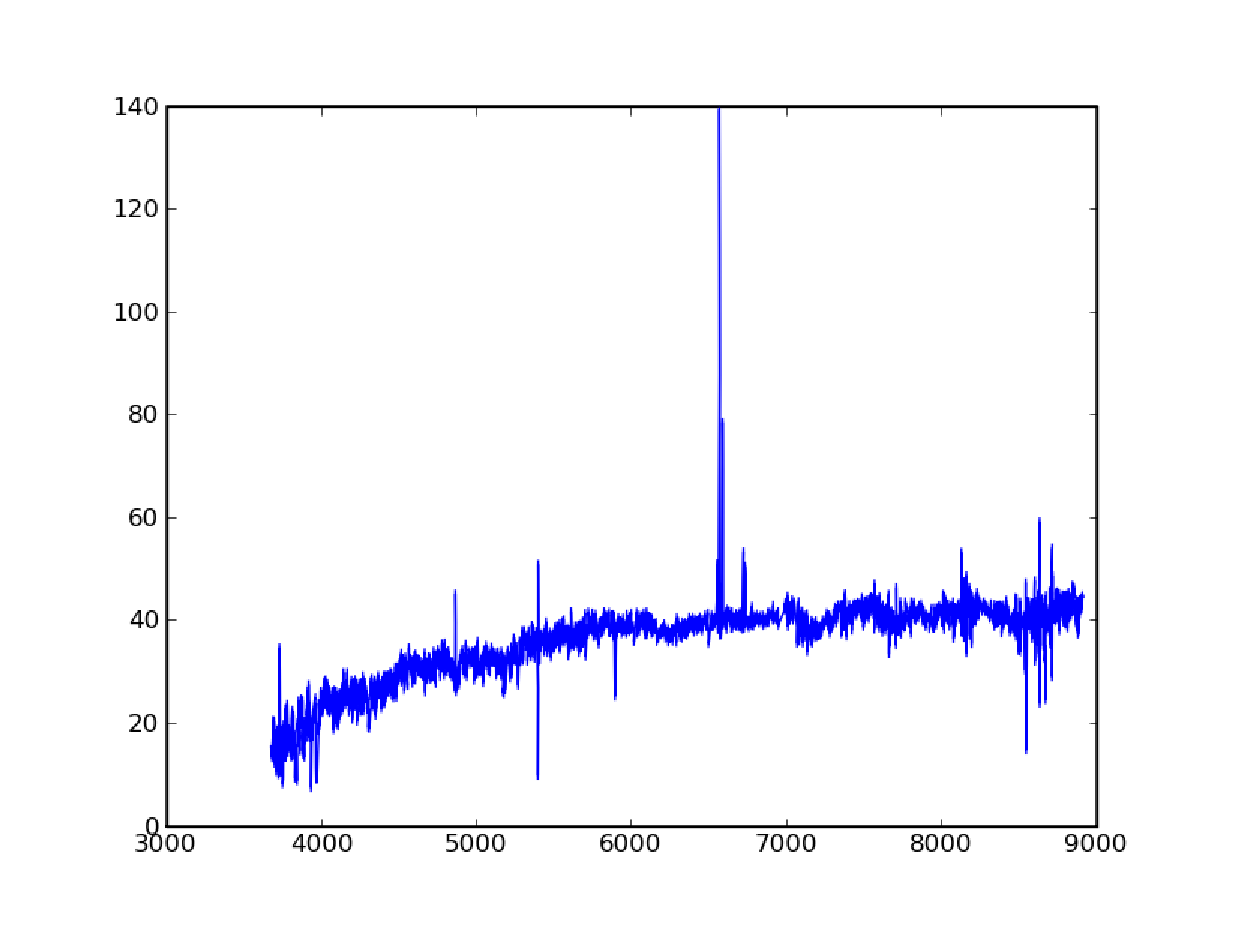
\includegraphics[width=1.\textwidth, height=.2\textheight]{spectra}\\

\vskip-2pt
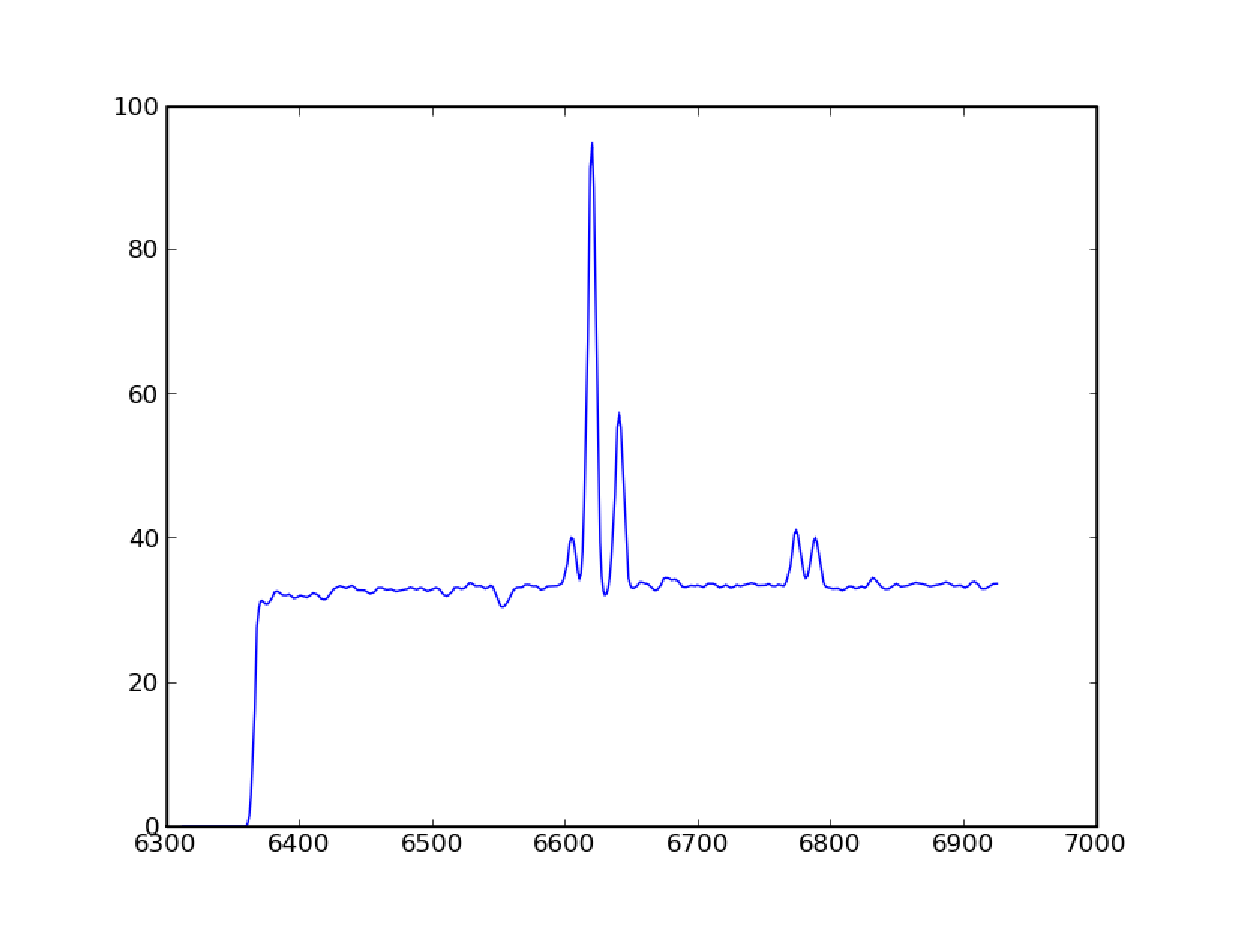
\includegraphics[width=.46\textwidth]{part}
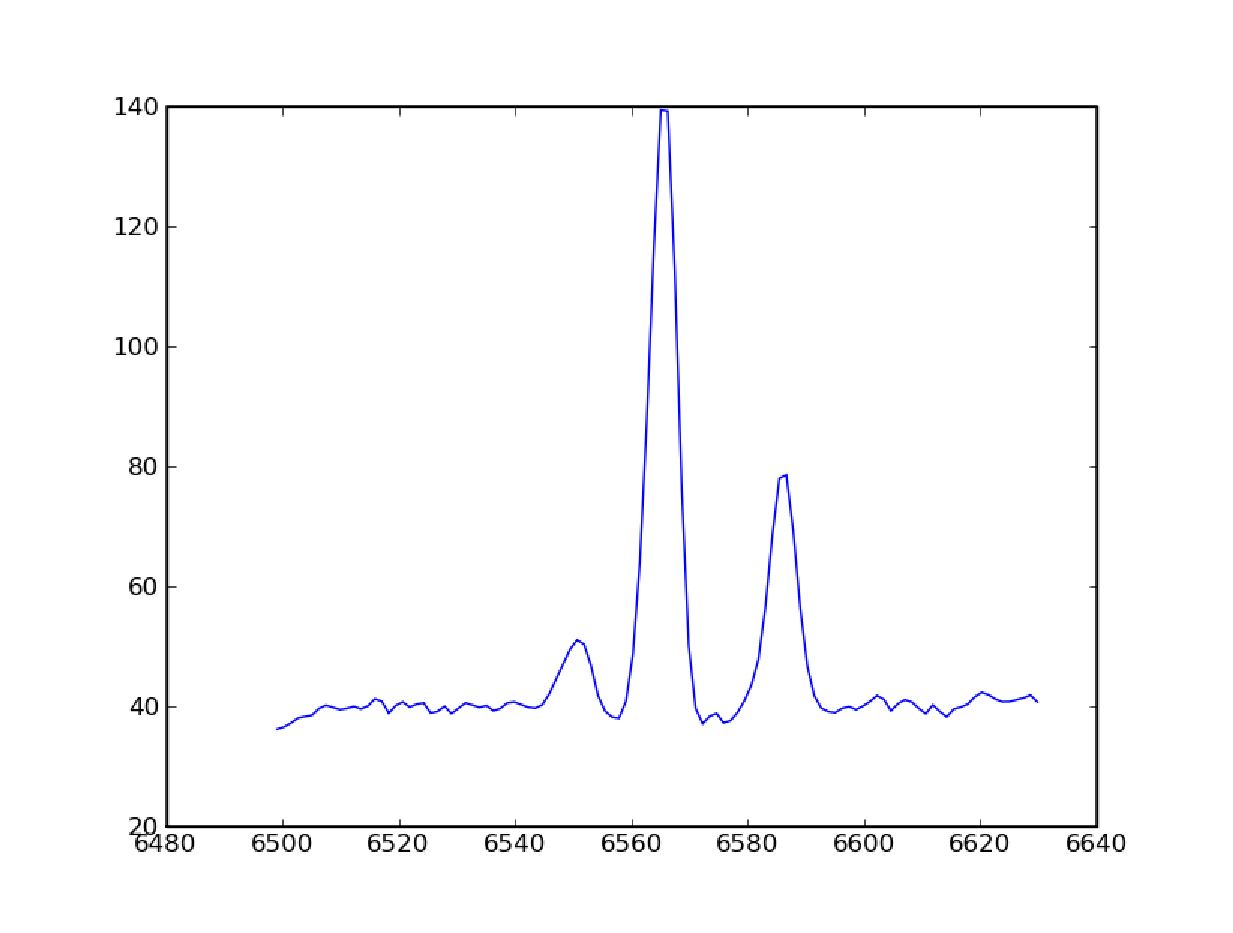
\includegraphics[width=.46\textwidth]{halpha}\\
The top one is the whole spectrum. Left bottom one is the spectrum after convolution by a gaussion kernel.Right bottom one is 
H$\alpha$ emission line.
\end{center}
\end{figure}
	  \section{Summary}
We introduces a new library for Python which can realize some functions of 
the ESO MIDAS. Using this library, people who are used to the gramma of the MIDAS
can keep their customs and enjoy the powful python. This library is for spectra
analysis. Because this is the first version of the library, not all the functions 
and commands of MIDAS are included. In the future, the library will be better.

\acknowledgements The ASP would like to the thank the dedicated researchers that are publishing with the ASP.


\end{document}
